\documentclass{SBCbookchapter}
\usepackage[utf8]{inputenc}
\usepackage[T1]{fontenc}
\usepackage[brazil,english]{babel}
\usepackage{graphicx}
\title{Typhoon Prediction: A Machine Learning Approach}
\begin{document}
\maketitle

%\addcontentsline{toc}{chapter}{Statistics}

%\emph{Find a statistical method which uses only Japan Meteorological Agency (JMA) best track typhoon data during or before year $n$ to hind-cast the entire best track of all typhoons in years $n+1$.   Given only the latter typhoons' initial three best track points (i.e. at $t=0,6,$ and $12$ hours), the maximum position error at each hind-casted track point must be less than 500 km. The method must work for the three most recent years of published best track data.}

\vspace{.3in}
\begin{minipage}[r]{4.25in}{\small
  The enormous devastation caused by super typhoon Haiyan (2013) motivates us to consider whether data from past typhoons might hold a key to predicting future typhoons.  Standard multiple-regression of historical
best track data (lat, lon, wind-speed, pressure given at 6 hr intervals) results in a simulated best track (SBT) for Haiyan with excessive position error. Whereas Haiyan's path was relatively straight, other typhoons have a curved path which makes prediction of typhoons from past data even more complicated.  CQN MQCHINE LEARNING BE USED to extract from past data the key to more accurate statistical prediction of super typhoon tracks?}
\end{minipage}

\newpage

\section{Introduction}

  In November 2013, Typhoon Haiyan struck the Philippines with sustained wind speeds of nearly 200
miles per hour, claiming over 6,000 lives, displacing 4 million people, damaging over a million houses,
and resulting in a request for over 750 million dollars
in humanitarian aid. Devastation caused by
``super typhoons" like Haiyan makes the on-going
development of early warning systems an absolute
necessity to provide vulnerable communities sufficient preparation time to
mitigate damage to both life and property. This motivated us to develop a regression model using data from recent typhoons which would closely simulate Haiyan's best track.

\section{A Basic Regression Model}
A basic multiple linear regression model which simulates a typhoon's best track at time steps $t_1, t_2, ....$ given at 6 hour intervals uses historical best track data for some time period (say 2009-2013) available from the Japan Meterological Agency's website http://www.jma. go jp/jma/jma-eng/jma-center/rsmc-hp-pub-eg/besttrack.html. This data is organized as shown in Table \ref{Table1}. At simulation time step $t_n$, the $k^{th}$ input data point $(t_{k,n},x_{k,n},y_{k,n},z_{k,n},w_{k,n})$ ($k=1,...,N$) specifies a best-track time ($t_{k,n}$), latitude ($x_{k,n}$), longitude ($y_{k,n}$), wind-speed ($z_{k,n}$) and pressure ($w_{k,n}$) of a historical typhoon, and the outputs are the latitude ($x_{k,n+1}$), longitude ($y_{k,n+1}$), wind-speed ($z_{k,n+1}$) and pressure ($w_{k,n+1}$) for the same typhoon 6 hours later, that is, at time $t_{k,n}+6$ (hrs).

\begin{table}[ht]
\scriptsize
\centering
\caption{ Data used in regression  (DUIR).}
\begin{tabular} {|ccccc|cccc|}
 \multicolumn{9}{c} { Data in the same row must come from the same historical typhoon. }\\\hline
 \multicolumn{5}{|c}{INPUT PREDICTOR DATA} & \multicolumn{4}{|c|}{OUTPUT PREDICTAND DATA}\\
 \multicolumn{5}{|c}{used in simulation step $n$} & \multicolumn{4}{|c|}{(Row $i$ data in this section is at time $t_{i,n}+6$ hr)}\\\hline
time (hr)  & latitude& 	longitude& 	intensity & pressure &	  latitude&longitude& intensity&pressure\\\hline
%\multicolumn{5}{c}}{}&\multicolumn{4}{c}{(row $i$ data at time $T_{i,n}+6} h \\\hline
$t_{1,n}$ & $x_{1,n}$&$y_{1,n}$& $z_{1,n}$ & $w_{1,n}$ & $x_{1,n+1}$&$y_{1,n+1}$& $z_{1,n+1}$ &$ w_{1,n+1}$ \\
$t_{2,n}$ & $x_{2,n}$&$y_{2,n}$& $z_{2,n}$ & $w_{2,n}$ & $x_{2,n+1}$&$y_{2,n+1}$& $z_{2,n+1}$ &$ w_{2,n+1}$ \\
\multicolumn{5}{|c|}{...}&  \multicolumn{4}{|c|}{...} \\
$t_{N,n}$ & $x_{N,n}$&$y_{N,n}$& $z_{N,n}$ & $w_{N,n}$ & $x_{N,n+1}$&$y_{N,n+1}$& $z_{N,n+1}$ &$ w_{N,n+1}$ \\\hline
\end{tabular}
\label{Table1}
\end{table}
\normalsize

{\flushleft This} data is used to obtain regression coefficients $a_i,b_i,c_i$, and $d_i$  ($i\in\{0,1,2,3,4,5\}$) by which we  obtain the simulated best track point $(X_{n+1},Y_{n+1},Z_{n+1},W_{n+1})$ at time $t_{n+1}$ given the current simulated best track point  $(X_{n},Y_{n},Z_{n},W_{n})$ at time $t_n$:

\begin{eqnarray}
X_{n+1} & = & a_0 + a_1 t_n + a_2 X_n + a_3 Y_n + a_4 Z_n + a_5 W_n \label{teq1}\\
Y_{n+1} & = & b_0 + b_1 t_n + b_2 X_n + b_3 Y_n + b_4 Z_n + b_5 W_n \label{teq2}\\
Z_{n+1} & = & c_0 + c_1 t_n + c_2 X_n + c_3 Y_n + c_4 Z_n + c_5 W_n \label{teq3}\\
W_{n+1} & = & d_0 + d_1 t_n + d_2 X_n + d_3 Y_n + d_4 Z_n + d_5 W_n. \label{teq4}
\end{eqnarray}

  {\flushleft A} simulated best track (SBT) is a sequence  $SBT_{n}=(X_{n},Y_{n},Z_{n}, W_n)$ ($n=0,1,2,3...$) generated by (\ref{teq1})-(\ref{teq4}). We used the actual typhoon's first 6 hour JMA best track data to initialize values for  $SBT_{0} = (X_{0}, Y_{0}, Z_{0}, W_0)$ at time $t_0=0$ and $SBT_{1}=(X_{1},Y_{1},Z_{1}, W_1)$ at time $t_1$=6 hr. (Using two points would give us the initial direction of the typhoon.)

  For the basic (``default'') multiple regression model, the data used in regression (DUIR) is fixed throughout the entire simulated best track. To simulate Haiyan, for exacmple,  the DUIR might be JMA grade 5 typhoons with Philippine landfall from 2009 up to the typhoon just before Haiyan. We found for different choices of DUIR, that this basic model gives a simulated best track for Haiyan with excessive error at the 120 hr or 5 day mark (Figure \ref{haiyanbasic}).

\begin{figure}[h]
\hspace{1.2in} 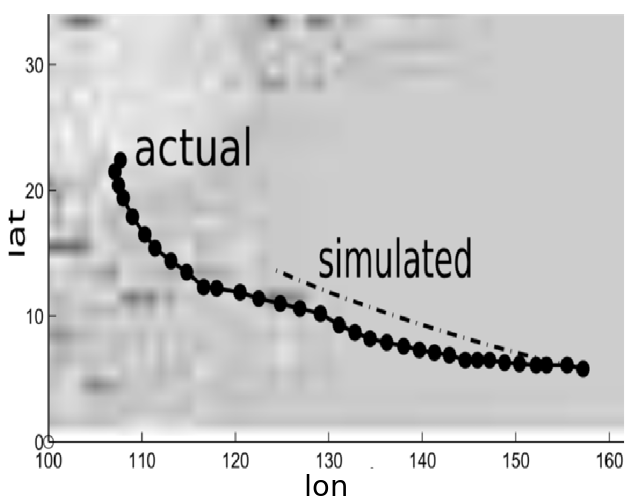
\includegraphics[width=4in, height=2.25in]{HaiyanTrackDefault.png}
 \caption{Default model simulation of Haiyan (2013) which exhibited a 1500 km track error at the 120 hr mark. See Table \ref{typ2}. }
 \centering
 \label{haiyanbasic}
\end{figure}



 \section{A p-norm Model Simulation of Haiyan}
 The simulated best track can be enhanced by filtering the DUIR by means of  a distance measure called a \emph{weighted $p-$norm}.
The $p$-norm model computes regression coefficients using a different subset of data from the DUIR at each time step by ordering the input data points by proximity to the current simulated best track point, and then using a fixed percentile of the ordered data. More specifically, at each time step $n$ of the SBT, we rank the rows of DUIR by degree of similarity to the current simulated track point $SBT_{n}=(X_{n},Y_{n},Z_{n}, W_n)$. We measure similarity of $SBT_n$ with the DUIR's $k^{th}$ row input data point  $ P_{k,n}=(x_{k,n}, y_{k,n},z_{k,n},w_{k,n})$ ($k=1,...,N$) by means of a weighted $p$-norm   defined by

          \begin{eqnarray*}
  \mid\mid P_{k,n} - SBT_n \mid\mid_{p} & = & \Big[\Omega_0 (\frac{t_{k,n}-t_n}{s_t})^p + \Omega_1(\frac{x_{k,n}-X_n}{s_x})^p + \Omega_2(\frac{y_{k,n}-Y_n}{s_y})^p+ \\
  && \Omega_3 (\frac{z_{k,n}-Z_n}{s_z})^p +  \Omega_4(\frac{w_{k,n}-W_n}{s_w})^p \Big]^{1/p},
  \label{pnorm}
        \end{eqnarray*}
        {\flushleft where}  $s_{_*}$ are standard deviations of the input data columns of the DUIR and $\Omega_*$ are the weights which are assumed for simplicity not to  depend on $n$. A $p$-norm model contains 4 different weighted $p$-norms and ranked percentiles, one for each of the 4 SBT coordinates (lat, lon, intensity, and pressure). Each weighted $p$-norm is specified by assigning the values of $p$ and the 5 weights ($\Omega_0,\Omega_1,\Omega_2,\Omega_3$, and $\Omega_4$). These parameters are used to rank the rows of DUIR by similarity to SBT$_n$. The values of  the ranked percentile parameters $\gamma_x$, $\gamma_y$, $\gamma_z$, $\gamma_w$ give the fractions of the ranked data used to obtain regression coefficients for each respective SBT coordinate.

        There are a total of 7$\cdot$4=28  parameters in a $p$-norm model.
        These parameters must be tuned using a specified training data set, such as all typhoons in 2013.  For the purpose of simulation, the best track data of the typhoon being simulated may be included in the parameter training data set.  For the purpose of prediction, only prior historical best-track data may be included in the training set.

                The term \emph{default parameters} denotes the special parameter set with all weights equal to 0 and all ranked percentiles equal to 1.  Using default parameters is equivalent to not using weighted $p$-norms since all the weights are zero. Moreover, the DUIR is neither ranked nor filtered since $\gamma_x=\gamma_y=\gamma_z=\gamma_w=1$.  In other words, a prediction using default parameters  is simply a basic multiple regression generated SBT on the original DUIR with neither rank ordering nor filtering of its rows.

          In our $p$-norm model, to obtain the regression coefficients $a_1,...,a_5$ needed to compute the next latitude coordinate $X_{n+1}$, we first use a latitude-specific weighted $p$-norm  to rank the rows in the DUIR by similarity to SBT$_n=(X_{n},Y_{n},Z_{n}, W_n)$. We then use $100\gamma_x\%$  (that is, the first  $N^*=\lfloor N\gamma_x \rfloor $ rows) of the ranked DUIR to create a matrix $\Gamma_{x,n}$ defined by
\begin{displaymath}
\Gamma_{x,n}=\left( \begin{array}{cccccc}
1 & t_{(1),n}&x_{(1),n}& y_{(1),n} & z_{(1),n} &w_{(1),n}\\
1 & t_{(2),n}&x_{(2),n}& y_{(2),n} & z_{(2),n} &w_{(2),n}\\
\multicolumn{6}{c}{...}\\
1 & t_{(N^*),n}& x_{(N^*),n}&  y_{(N^*),n} & z_{(N^*),n} &w_{(N^*),n}\\
\end{array}
\right ),
\end{displaymath}
{\flushleft where subscript parentheses} indicate data ranked by weighted $p$-norm similarity.  Defining the vector  $\stackrel{\rightarrow}{\phi}_{x,n}=(x_{(1),n+1}, x_{(2),n+1},..., x_{(N^*),n+1})^{\tau}$ ($\tau=$ transpose), we  obtain the latitude regression coefficients as components of the vector
\begin{eqnarray}
\stackrel{\rightarrow}{A}_{x,n}& = &(\Gamma_{x,n}^{\tau}\Gamma_{x,n})^{-1}\Gamma_{x,n}^{\tau}\stackrel{\rightarrow}{\phi}_{x,n} \label{regeq1}\\
  &= &(a_{0,n},a_{1,n},a_{2,n},a_{3,n},a_{4,n},a_{5,n})^{\tau}.\nonumber
\end{eqnarray}

In a similar way, for the longitude, intensity and pressure regression coefficients we use respectively longitude-, intensity- and pressure-specific weighted $p$-norms, ranked DUIR and percentile parameters $\gamma_y,\gamma_z$ and $\gamma_w$ to construct matrices $\Gamma_{y,n}$,$\Gamma_{z,n}$ and $\Gamma_{w,n}$. We then define vectors  $\stackrel{\rightarrow}{\phi}_{y,n}, \stackrel{\rightarrow}{\phi}_{z,n}$ and $\stackrel{\rightarrow}{\phi}_{w,n}$ and compute the longitude $\stackrel{\rightarrow}{B}_{y,n}$, intensity $\stackrel{\rightarrow}{C}_{z,n}$ and pressure $\stackrel{\rightarrow}{D}_{w,n}$ regression coefficient vectors as before. Finally, these regression coefficients are used to obtain the next simulated best track point  $SBT_{n+1}$ using (\ref{teq1})-(\ref{teq4}).

To simulate typhoon Haiyan, we initialize the SBT using Haiyan's initial data $SBT_0=(X_0,Y_0,Z_0,W_0)=(5.8, 157.2, 0, 1004)$ and  $SBT_1=(X_1,Y_1,Z_1,W_1)$=(6.1, 155.5,0,1008).  The parameter set in Table \ref{typ2}  was obtained by  a training session to minimize the mean 120-hr track error for the 4 Philippine-landfall, JMA Grade 5 typhoons in 2013  (mean error = 441.7 km. for the parameters in Table 2.)     Specifying our DUIR to be JMA best track grade 5 Philippine landfall typhoon data from 2009 up to Haiyan, Table \ref{typ2} shows, the $p$-norm model SBT for Haiyan reduces the default parameter's 5-day track error by over 1,300 km.

    \begin{table}[h]
\centering
\tiny
\begin{tabular}{|l|l|l|l|l|l|l|l|l|}
\multicolumn{9}{c}{$p$-NORM MODEL PARAMETERS }\\\hline
&$\Omega_0$ & $\Omega_1$ & $\Omega_2$ & $\Omega_3$ & $\Omega_4$ & $p$ &\multicolumn{2}{l|}{$\gamma$}\\\hline
Latitude &  .5 & 25 & .25 & 59.5 & 0 & 1.3 & \multicolumn{2}{l|}{.05} \\
Longitude &  0 & 0 & 0 & 0 & 0 & 0 & \multicolumn{2}{l|}{.35} \\
Intensity &  .01 & 1 & 10 & 5 & 0 & 1.2 & \multicolumn{2}{l|}{.2} \\
Pressure & .4 &1000&.65&20&5&1.1&\multicolumn{2}{l|}{.6} \\ \hline \hline
\multicolumn{9}{|c|}{POSITION ERRORS }\\\hline
  Hours in advance    & 24-hr & 48-hr &72-hr &96-hr & 120-hr & 144-hr & 168-hr& 192-hr\\\hline
  Default position error  (km)  &297.6  &477.3 & 728.0&1021.9 & 1498.8 &1874.3  & 2105.0 &  1975.6 \\\hline
  $p$-norm position error  (km)   &  125.1  &  97.2  & 46.6  & 65.5  & 167.3& 266.7  &  445.1&   634.6   \\\hline
  Relative error reduction & $R_1=.58 $  &$R_2=.8 $ &$R_3=.94 $ &$R_4=.94 $ &$R_5=.89 $ &$R_6=.86 $  &$R_7=.79 $ &  $R_{7.75} =.68 $   \\ \hline
 \end{tabular}
  \caption{Haiyan (international ID 1330) $p$-norm model simulation. DUIR: JMA grade 5 Philippine landfall (2009 up to Haiyan) }
  \label{typ2}
\end{table}
%\begin{figure}[h]
%\centering
% \includegraphics[width=4in, height=2.25in]{TyphoonSimulation/HaiyanWSDC3.png}
% \caption{Track error in the Haiyan (2013) default model is reduced by the $p$-norm model; parameters given in Table 2.)}
% \label{haiyanp}
%\end{figure}



  {\flushleft Table} \ref{typ2} also gives the relative reduction of the default position error by the $p$-norm model, namely, $R_n=1 - \frac{\epsilon_n  }{\delta_n  }$,  where $\epsilon_n$ is the $p$-norm model error and $\delta_n$ the default parameter model error $n$ days after time $t_1=6$ hr.  Note that $R_n=1$ if the $p$-norm model error is 0;    $R_n=0$ if the $p$-norm and default parameter model  errors are the same;  and $R_n<0$ if the $p$-norm model error is larger than the default parameter model. If $R_n>0$, the $p$-norm model reduces the default error by $100R_n\%$.



Though Haiyan travelled an essentially straight path, another super typhoon, Guchol (2012) followed a highly curved path, and was mentioned in \cite{JMA} as being particularly problematic in its best track forecast.    This curvature, missing in the basic regression model, is simulated well by inclusion of weighted $p$-norms.   Referring to Table \ref{typ3}, the $p$-norm model reduces   Guchol's SBT 168-hr (7-day) error to 159.1 km ($R_{7}=79\%$) (Figure \ref{gucholfig}.)

  \begin{table}[h]
\centering
\tiny
   \begin{tabular}{|l|l|l|l|l|l|l|l|}
\multicolumn{8}{c}{$p$-NORM MODEL PARAMETERS }\\\hline
$p$-norm model parameters&$\Omega_0$ & $\Omega_1$ & $\Omega_2$ & $\Omega_3$ & $\Omega_4$ & $p$ &$\gamma$\\\hline
Latitude &  5 & 9.5 & 20 & .2 & 1 & 1.73 & .26 \\
Longitude &  9 & 25 & 15 & .3 & 0 & .5 & .95 \\
Intensity &  20 & 1 & 10 & 5 & 0 & 1 & .5 \\
Pressure & 1 &10&15&15&12.5&1.1&.85 \\ \hline \hline
\multicolumn{8}{|c|}{POSITION ERRORS }\\\hline
  Hours in advance   & 24-hr & 48-hr &72-hr &96-hr & 120-hr &   144-hr& 168-hr\\\hline
 Default position error  (km)&  15.3  & 140.4    & 31.6  & 198.2   & 203.1 &  341.0 &747.1 \\\hline
 $p$-norm position error  (km)&  37.8  &  150.0  & 162.9  & 416.2  &  390.1& 151.1&159.1 \\\hline
 Relative error reduction & $R_1= -1.47 $  &$R_2=-.07 $ &$R_3=-4.16 $ &$R_4=-1.1 $ &$R_5=-.92 $ &$R_6=.56 $  &$R_7=.79 $ \\ \hline \hline
   Hours in advance   &  192-hr &216-hr & 240-hr &  264-hr & 288-hr &  312-hr & 336-hr \\\hline
 Default position error  (km)    & 1257.1  & 1892.1   & 2722.0 &3343.9  & 4140.6    & 4659.2  & 5088.5     \\\hline
 $p$-norm position error  (km)  & 348.3  & 647.7  &  1096.9&   1284.4  &  1548.0  & 1473.7  & 1126.3       \\\hline
 Relative error reduction & $R_8=.72 $ &$R_9=.66 $ &$R_{10}=.62 $   & $R_{11}=.60 $  &$R_{12}=.62 $ &$R_{13}=.68 $ &$R_{14}=.78$ \\ \hline \hline
 \end{tabular}
  \caption{Guchol (international ID 1204) $p$-norm model simulation. DUIR:  JMA best track grade 5 typhoon data (2009-)}
  \label{typ3}
 \end{table}
\begin{figure}[h]
\centering
  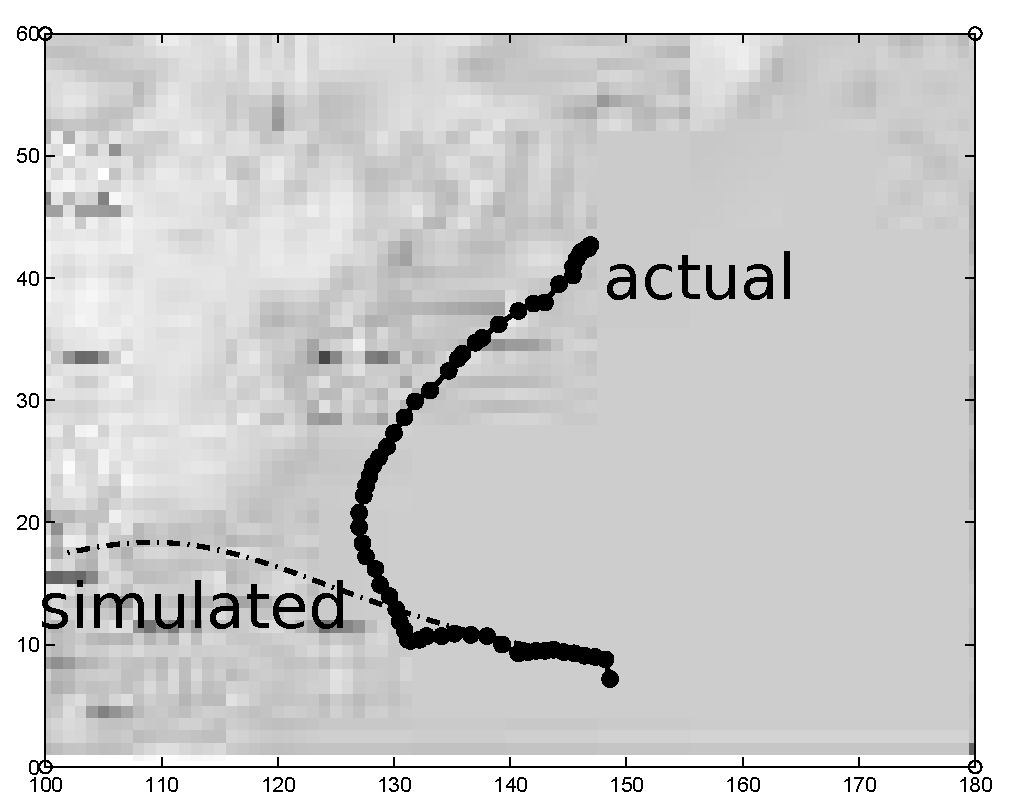
\includegraphics [width=2.5in, height=2.25in]{GucholTrackDefault.eps}
  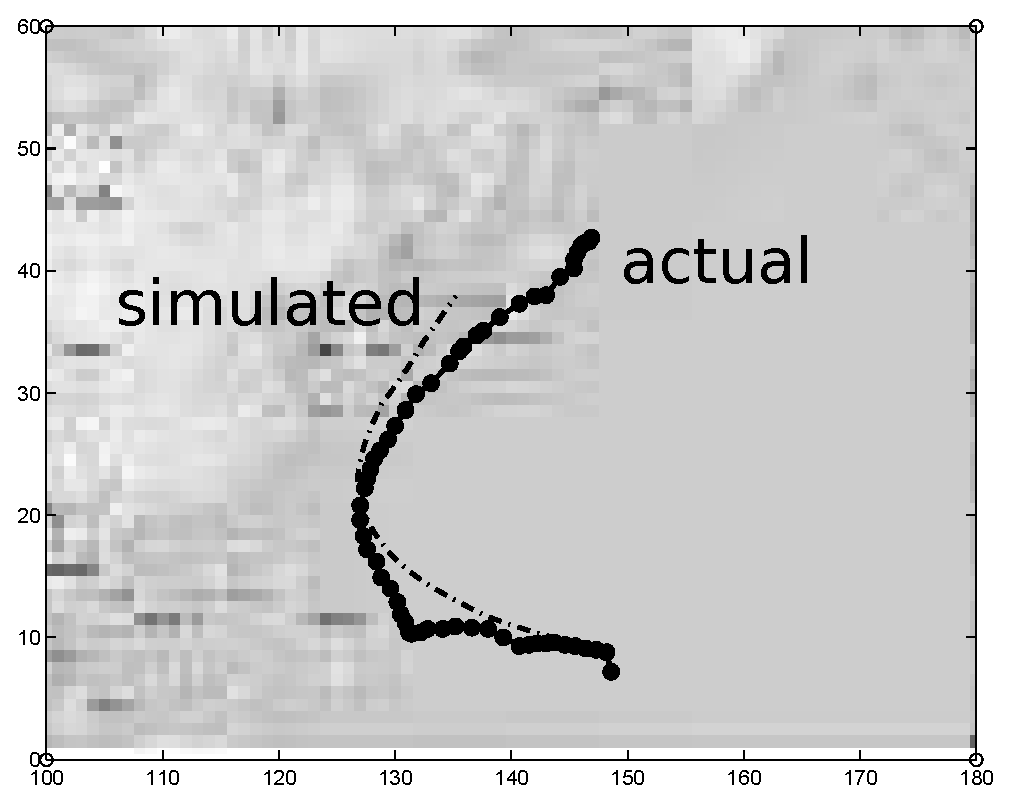
\includegraphics[width=2.5in, height=2.25in]{GucholTrackp.eps}
     \caption{Missing curvature in the default model of Guchol (2012) is corrected by the $p$-norm model (solid markers=actual, dashed=simulated; parameters given in Table 3.)}
  \label{gucholfig}
\end{figure}



\section{Annual Forecasting}
     Simulations of Hayian and Guchol suggest the potential of a $p$-norm model to forecast an emerging typhoon. The difficulty, however, is finding the best parameter set using training data that is historical prior to the storm being predicted. Moreover, the same parameter set ideally will work well on average for all typhoons occurring in the same typhoon season (year).

          We illustrate what is called ``quasi-operational prediction'' or ``hind-casting'' using the thirteen typhoons occurring in 2013 as a parameter training set, and then checking how well the $p$-norm model works on predicting (``hind-casting") all eleven typhoons in 2014.  Using 2013 data as the DUIR and given only the initial best track data of each 2014 typhoon,   the $p$-norm model reduces the default model's  mean 2014 typhoon 120-hr position error from 1258 km to 1088 km (Table \ref{typ5}).

%
% \begin{table}[h]
%\centering
%\scriptsize
%   \begin{tabular}{|l|l|l|l|l|l|l|l|}
%\multicolumn{8}{c}{$p$-NORM MODEL PARAMETERS }\\\hline
%$p$-norm model parameters&$\Omega_0$ & $\Omega_1$ & $\Omega_2$ & $\Omega_3$ & $\Omega_4$ & $p$ &$\gamma$\\\hline
%Latitude &  0 & 15 & 70 & 7.5 & 1 & 1 & .895 \\
%Longitude &  0 & 0 & 0 & 0 & 0 & 0 & .29 \\
%Intensity &  2.5 & .5 & 100 & 5 & 3.2 & .1 & .2 \\
%Pressure & 1 &.845&3&15&12.5&1.1& .85 \\\hline\hline
%\multicolumn{8}{|c|}{POSITION ERRORS }\\\hline
%\multicolumn{8}{|c|}{2013 Training simulations (13 JMA grade 5 typhoons)}\\ \hline
%\multicolumn{3}{|l|}{  Hours in advance}   & 24-hr & 48-hr &72-hr &96-hr & 120-hr\\\hline
%\multicolumn{3}{|l|}{  Mean default position error  (km)}  &291.0  &511.2 &718.5 & 928.9& 1148.9 \\\hline
%\multicolumn{3}{|l|}{  Mean $p$-norm position error  (km)}  & 267.6 &456.6 & 625.2& 768.1& 961.9 \\\hline
%\multicolumn{3}{|l|}{  Relative error reduction} & $R_1= .08 $  &$R_2=.11 $ &$R_3= .13$ &$R_4= .17 $ &$R_5= .16$  \\\hline\hline
%\multicolumn{8}{|c|}{2014 Quasi-operational forecasts (11 JMA grade 5 typhoons)}\\ \hline
% \multicolumn{3}{|l|}{  Hours in advance}   & 24-hr & 48-hr &72-hr &96-hr & 120-hr \\\hline
%\multicolumn{3}{|l|}{  Mean default position error  (km)} & 242.1 & 411.3    &640.5 & 965.2&1257.6  \\\hline
%\multicolumn{3}{|l|}{  Mean $p$-norm position error  (km)}  &214.5  &361.9     &539.6 &816.0 & 1088.0 \\\hline
%\multicolumn{3}{|l|}{  Relative error reduction} & $R_1= .11 $  &$R_2= .12$ &$R_3= .16$ &$R_4=.15 $ &$R_5=.13 $ \\ \hline\hline
%\end{tabular}
%\caption{2013 season training simulation (13  typhoons)/2014 season quasi-operational forecast (11 typhoons) DUIR: JMA best track typhoon data (2009-)}
%\label{typ4}
%\end{table}
%
%        \newpage
 {\flushleft Observing} a substantial error reduction in 8 out of the 11 typhoons and a mean reduction of 13\% demonstrates the $p$-norm model's ability to improve upon default model hind-casting.
\begin{table}[!htpb]
\scriptsize
\centering
   \begin{tabular}{|c|l||c|c|c|}\hline
 Super& International&\multicolumn{2}{|c|}{120-h Error}& Reduction\\
      Typhoon  & I.D. &Default & $p$-norm & R$_5$\\\hline
 Faxai&1403&2230.3&2442.6&(-.1)\\\hline
 Neoguri& 1408&932.5&795.7&.15$^*$\\\hline
 Rammasun &1409&1148.6&662.1  &.42\\\hline
 Matmo& 1410&848.1&920.1&(-.08)\\\hline
 Halong  & 1411&641.0 &383.0& .40\\\hline
 Genevieve  & 1413&2143.0 &1594.3& .26\\\hline
 Kalmaegi&1415&1613.4 &1709.0& (-.06)\\\hline
 Phanfone   & 1418&1283.1 &1118.4& .13\\\hline
 Vongfong &  1419&1481.1 &1250.0&.16\\\hline
 Nuri & 1420&915.8 & 870.1&.05\\\hline
 Hagupit& 1422&597.1&222.9&.63\\\hline\hline
\multicolumn{2}{|r|}{MEAN (11 typhoons)}&1257.6 &  1088.0& .13 \\\hline
\multicolumn{5}{r}{$^*${\tiny missing curvature corrected}}
  \end{tabular}
  \caption{  2014 $p$-norm model 120-hr error reductions.}
  \label{typ5}
 \end{table}

In contrast to the prevailing big data typhoon forecasting models, the basic and $p$-norm regression models use only a subset of a small (1 megabyte) data set consisting of Japan Meteorological Agency (JMA) typhoon best track data from 2009-2014. Thus, our best tracks can easily be simulated on a personal laptop. On the other hand, the 120-hr mean 2014 position error of 1088 km for the $p$-norm model is roughly double JMA's operational (``live'') typhoon prediction error. The latter uses the most sophisticated statistical methods, global weather data assimilation on supercomputers, and advanced knowledge of mathematical physics to achieve an annual mean 5-day forecasted position error of roughly 500 km. Even so,  the JMA  has `busted cases'  with large predicted track position errors similar in size to our default model's simulation of Haiyan \cite{Ito}. Thus, professional typhoon forecasters must keep the door open for new approaches to improve accuracy of long-range forecasting models which have the greatest humanitarian benefit. Is there a way to use just historical typhoon data to match the current standard of long-range operational typhoon prediction accuracy?



\section{Exercises}

 \begin{enumerate}
\item Let $p=2$ and $\Omega_i=1$ for all $i$. Show the following: a) $||A-B||_p \ge 0$;  b)  $||A-B||_p = 0$ if and only if $A=B$.
 \item Use partial derivatives and minimization of sum of squared residuals to derive equation (\ref{regeq1}).
 \item Analyze whether the reduction in position error in Table \ref{typ5} is significant.
     \item Write a paper reviewing the history of statistical typhoon forecasting  (see, for example, \cite{Arakawa}).
\item  Does the highly active research field called \emph{statistical learning} (which includes machine learning) offer new approaches for statistical typhoon forecasting?
\item One idea to simplify the prediction of super typhoons like Haiyan is to focus on prediction of just the most violent points (MVPs) (i.e. points with wind speed at least 105 km)  using historical data for just the genesis points (GPs) (i.e. best track points at $t=0$) and MVPs of recent JMA Grade 5 typhoons. Build a multiple regression model to hindcast MVPs from GPs (see Figure \ref{GPMVP}). Describe the structure of your DUIR, type of training sets utilized, and hind-casted MVP position errors. How can a Monte Carlo simulation be used to assess your model's mean MVP position prediction error?
\end{enumerate}

\begin{figure}[!htpb]
 \centering
\includegraphics[width=5.in,height=3.in]{violentfig3.eps}
\caption{Genesis points (GPs) and most violent points (MVPs) of 2009-2012 Grade 5 typhoons. GP Window:[134.7$^o$E x 160.4$^o$E]x [6.7$^o$N,14.3$^o$N]; MVP Window: [123.3$^o$E x 145.0$^o$E]x [13.6$^o$N,19.2$^o$N]}
\label{GPMVP}
\end{figure}

\newpage

\section{Computer Project}
Write a program which can create SBTs for the default and $p$-norm models such as shown in Figure \ref{gucholfig}.





\vspace{1in}

\emph{Acknowledgement:} Guidance from Dr. Takemasa Miyoshi and the Journal of the Meteorological Society of Japan's editorial staff is gratefully acknowledged. This project was supported by Wheaton College's Summer Research Programs.
.
\vspace{.25in}

\emph{Project Team:} Korey Clement, Daniela Cuba, Michael Kietzman, Peyton Finley, Jacob Clement, Danilo Diedrichs, Roland Hesse, Spencer Hills, Kaile Phelps, Jenny Ruda, Erica Swain, Kei Takazawa, Emily Wilson

\newpage
 \begin{thebibliography}{9}

 \bibitem{Arakawa}  {\sc  ARAKAWA, H.}, 1964. Statistical method to forecast the movement and the central pressure of typhoons in the western north Pacific. \emph{J. Appl. Meteorol.} {\bf 3}, 524-528.

     \bibitem{Cap}   {\sc CAP, F.}, 200.: {\em Tsunamis and Hurricanes: A Mathematical Approach.} Springer-Verlag, 201 pp.

\bibitem{Chan} {\sc CHAN, J.C.L.}, 2005: The physics of tropical cyclone motion. \emph{Annu. Rev. Fluid Mech.} {\bf 37}, 99-128.
\bibitem{Hig}  {\sc HIGAKI, M.}, {\sc KYOUDA, M.} and {\sc YAMAGUCH, H.} 2015. Upgrade of JMA's Typhoon Ensemble Prediction System. http://www.wcrp-climate.org/ WGNE/ Blue Book/2014/individual-articles/06\_Higaki\_Masakazu\_  \\WGNE\_BB2014\_TEPSupgrade\_higaki.pdf



\bibitem{Ito}   {\sc  ITO, K. } and  {\sc WU, C.   }, 2013. \emph{Typhoon-position-oriented sensitivity analysis. part I: theory and verification. } \emph{J. Atmos. Sci.}, {\bf 70}, 2525-2546.

    \bibitem{JMA} {\sc JAPAN METEORLOLOGICAL AGENCY}, 2014: \emph{Annual Report of the RSMC Tokyo-Typhoon Center 2013}. http://www.jma.go.jp/jma/ jma- eng/jma-center/rsmc-hp-pub-eg/AnnualReport/2013/Text/Text2013.pdf

\bibitem{Neumann} {\sc NEUMANN, C. J.}, 1972. \emph{An alternate to the HURRAN tropical cyclone forecast system.} \emph{NOAA Tech. Memo.} NWS SR-62, 22 pp.

\end{thebibliography}

%\item  Arakawa, H., 1964: Statistical method to forecast the movement and the central pressure of typhoons in the western north Pacific.  \emph{J. Appl. Meteorol.} {\bf 3}, 524-528.
%

%    \item Ito, K. and C. Wu, 2013: Typhoon-position-oriented sensitivity analysis. part I: theory and verification. \emph{J. Atmos. Sci.}, {\bf 70}, 2525-2546.

%
%
%\vspace{.2in}
%
%\scriptsize
%{\flushleft \bf References}
%
%\begin{list}{}{\leftmargin=1em \itemindent=-2em}
%
%\item Anthes, R.A., 1982: \emph{Tropical cyclones. Their evolution, structure and effects.} American Meteorological Society.208 pp.
%

%
%\item Cap, F. 2006: {\em Tsunamis and Hurricanes: A Mathematical Approach.} Springer-Verlag, 201 pp.
%
%\item Cecelski, S.F., D.-L. Zhang and T. Miyoshi, 2014: Genesis of hurricane Julia (2010) within an African easterly wave: developing and non-developing members from ERF-LETKF ensemble forecasts. \emph{J. Atmos. Sci.}, {\bf 71}, 2763-2781.
%
%\item Chan, J.C.L., 2005: The physics of tropical cyclone motion. \emph{Annu. Rev. Fluid Mech.} {\bf 37}, 99-128.
%
%\item Chan, J.C.L., 2010: Movement of Tropical Cyclones. \emph{Global Perspectives on Tropical Cyclones: From Science to Mitigation}, J.C.L. Chan and J.D. Keperts, eds., World Scientific Publishing, 133-148.
%
%
%\item  Chang, C.-C., S.-C. Yang and C. Keppenne, 2014: Applications of the mean recentering scheme to improve typhoon track prediction:  a case study of typhoon Nanmadol (2011). \emph{J. Meteor. Soc. Japan} {\bf 92}, 559-584.
%
%
%
%\item Elsberry, R., 1995: Tropical cyclone motion. \emph{Global Perspectives on Tropical Cyclones}, J.C. L. Chan and J.D. Kepert, Eds., World Meteorological Organization, 106-197.
%
%\item Epstein, E.S., 1969: Stochastic dynamics prediction. \emph{Tellus}, {\bf 21}, 739-759.
%
%
%\item Higaki, M., M. Kyouda and H. Yamaguchi, 2015: Upgrade of JMA's Typhoon Ensemble Prediction System. http://www.wcrp-climate.org/ WGNE/ Blue Book/2014/individual-articles/06\_Higaki\_Masakazu\_  \\WGNE\_BB2014\_TEPSupgrade\_higaki.pdf
%
%
%\item Hope, J. R. and C.J. Neumann, 1970: An operational technique for relating the movements of existing tropical cyclones to past tracks. \emph{Mon. Weather Rev.}, {\bf 98}, 925-933.
%
%
%    \item Ito, K. and C. Wu, 2013: Typhoon-position-oriented sensitivity analysis. part I: theory and verification. \emph{J. Atmos. Sci.}, {\bf 70}, 2525-2546.
%
%
%\item Japan Meteorological Agency, 2013: {\em Annual Report of the RSMC Tokyo-Typhoon Center 2012}. http://www.jma.go.jp/jma/ jma- eng/jma-center/rsmc-hp-pub-eg/AnnualReport/2012/Text/Text2012.pdf
%
%\item Japan Meteorological Agency, 2014: {\em Annual Report of the RSMC Tokyo-Typhoon Center 2013}. http://www.jma.go.jp/jma/ jma- eng/jma-center/rsmc-hp-pub-eg/AnnualReport/2013/Text/Text2013.pdf
%
%
%\item Jin, L., C. Yao and X. Huang, 2008: A Nonlinear Artificial Intelligence Ensemble Prediction Model for Typhoon Intensity. \emph{Mon. Weather Rev.}, {\bf 136}, 4541-4554.
%
%\item Knaff, J.A., C.R. Sampson, and M. DeMaria, 2005: An operational statistical intensity prediction scheme for the western north Pacific. \emph{Weather Forecast.}, {\bf 20}, 688-699.
%
%
%    \item Komaromi, W.A., S.J. Majumdar and E.D. Rappin, 2011: Diagnosing initial condition sensitivity of typhoon Sinlaku (2008) and hurricane Ike (2008), {\bf 139}, 3224-3241.
%
%\item  Korean Meteorological Administration, 2013: {\em Annual Report}. \\ http://web.kma.go.kr/download\_01/Annual\_Report\_2013.pdf
%
%\item Krishnamurti, T.N., J. Xue, H.S. Bedi, K. Ingles, and D. Oosterhof, 1991: Physical initialization for numerical weather prediction over the tropics. \emph{Tellus}, {\bf 43}, 53-81.
%
%\item Krishnamurti, T.N., C.M. Kishtawal, T.E. LaRow, D.R. Bachiochi, Z. Zhang, C.E. Williford, S. Gadgil, and S. Surendran, 1999: Improved weather and seasonal climate forecast from multi-model superensemble. \emph{Science}, {\bf 285}, 1548-1550.
%
%\item Leith, C.E., 1974: Theoretical skill of Monte-Carlo forecasts. \emph{Mon. Wea. Rev.,} {\bf 102}, 409-418.
%
%\item Leslie, L.M., R. Abbey and G.J. Holland, 1998. Tropical cyclone track predictability. \emph{Meteorol. Atmos. Phys.}, {bf 65}, 223-231.
%
%\item Lorenz, E.N., 1963: Deterministic nonperiodic flow. \emph{J. Atmos. Sci.}, {\bf 20}, 130-142.
%\item Lorentz, E.N., 1965: A study of the predictability of a 28-variable atmospheric model. \emph{Tells}, {\bf 17}, 321-333.
%
%\item Meng, Z. and F. Zhang, 2007: Tests of an ensemble Kalman filter for mesoscale and regional-scale data assimilation. Part II: Imperfect model experiments. \emph{Mon. Weather Rev.,} {\bf 135}, 1403-1423.
%
%\item Neumann, C. J., 1972: An alternate to the HURRAN tropical cyclone forecast system. \emph{NOAA Tech. Memo.} NWS SR-62, 22 pp.
%
%\item  Rozanova, O. S., J.-L. Yu, and C.-K. Hu, 2010: Typhoon eye trajectory based on a mathematical model: comparing
%with observational data. \emph{Nonlinear Analysis: Real World Applications.} {\bf 11}, 1847�1861.
%
%\item $\ddot{\textup{U}}$ster, H. and R.F. Love, 2001: Application of a weighted sum of order $p$ to distance estimation. \emph{IIE Trans.}, {\bf 33}, 675-684.
%
%\item Weber, H., 2005: Probabilistic prediction of tropical cyclones. part 1: position. \emph{Mon. Weather Rev.}, {\bf 133}, 1840-1852.
%
%\item Williford, C.E., T.N. Krishnamurti, R.C. Torres, and S. Cocke, 2003: Real-time multimodel superensemble forecasts of Atlantic tropical systems of 1999. \emph{Mon. Weather Rev.}, {\bf 131}, 1878-1894.
%
%\item Wu, C.-C., and K. Emmanuel, 1993: Interaction of baroclinic vortex with background shear: application to hurricane movement. \emph{J. Atmos. Sci.}, {\bf 50}, 62-76.
%
%    \item Yamaguchi, M., T. Nakazawa, and K. Aonashi, 2012:  Tropical Cyclone track forecasts using JMA model with ECMWF and JMA initial conditions. \emph{Geophys. Rev. Lett.,} {\bf 39}, L09801, doi:10.1029/2012GL051473.
%
%\item Yanase, W., H. Taniguchi, M. Satoh, 2010: The genesis of tropical cyclone Nargis (2008): environmental modulation and numerical probability. \emph{J. Meteor. Soc. of Japan}, {\bf 88}, 407-519.
%
%        \item Yang, S.-C., E. Kalnay and T. Miyoshi, 2012: Accelerating the EnKF spinup for typhoon assimilation and prediction. \emph{Weather Forecast.}, {\bf 27}, 878-897.
%
%\end{list}

%Official annual tropical storm and typhoon best track data (lat, lon, windspeed, pressure in 6 hour time increments) is published by the Japan Meteorological Agency (JMA). To develop a best track prediction model, you are allowed to use as your training data the JMA best track data for the thirteen typhoons Soulik, Utor, Manyi, Usagi, Wutip, Fitow, Dana, Nari, Wipha, Francisco, Lekima, Krosa, and Haiyan in 2013  available at
%  \\ {\scriptsize http://www.jma.go.jp/jma/jma-eng/jma-center/rsmc-hp-pub-eg/besttrack.html}.
%{\flushleft Design} a model such that given just the 2013 training data and the initial best track point of the eleven typhoons in 2014 shown in the table below, you can predict the best track position of each 2014 typhoon at the 120 hour mark with an average error of less than 500 km.
%
%\begin{table}[!htpb]
%\scriptsize
%\centering
%\begin{tabular}{|c|l||c|c|c|c|}\hline
% Typhoon& International&\multicolumn{4}{|c|}{Initial best track}\\
%        & I.D. &lat & lon & pressure  & wind speed\\\hline
% Faxai&1403&8.7&147.8&1004&0\\\hline
% Neoguri& 1408&8.4&146.8&1006&0\\\hline
% Rammasun &1409&8.0&154.3  &1006&0\\\hline
% Matmo& 1410&10.0&136.8&1006&0\\\hline
% Halong  & 1411&11.3 &151.8& 1006&0\\\hline
% Genevieve  & 1413&13.6 &181.2& 950&0\\\hline
% Kalmaegi&1415&13.5 &134.0&1004&0\\\hline
% Phanfone   & 1418 &11.0& 157.1&1004&0\\\hline
% Vongfong &  1419&7.3 &162.1&1006&0\\\hline
% Nuri & 1420&12.6 & 140.9&1004&0\\\hline
% Hagupit& 1422&2.6&156.0&1006&0\\\hline\hline
%  \end{tabular}
%  \caption{ Initial best track points of typhoons in 2014.}
%  \end{table}
%
%\vspace{.3in}
%
%
\end{document}